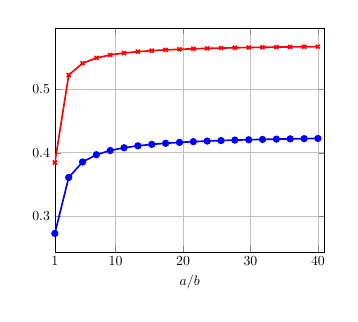
\begin{tikzpicture}[scale=0.5]
\begin{axis}[xlabel=$a/b$,ymajorgrids=true,xmajorgrids=true,xmin=1,xmax=41,xtick={1,10,20,30,40}]
%%%%%%%%%%% NATURAL CONFIGURATION
\addplot[Blue,mark=*,very thick] coordinates {(1.0,0.272727272727) (3.05263157895,0.360995850622) (5.10526315789,0.385430463576) (7.15789473684,0.396887159533) (9.21052631579,0.403535741737) (11.2631578947,0.407878017789) (13.3157894737,0.410936654034) (15.3684210526,0.41320754717) (17.4210526316,0.414960300878) (19.4736842105,0.416354088522) (21.5263157895,0.417488941817) (23.5789473684,0.418430884184) (25.6315789474,0.419225251076) (27.6842105263,0.419904204364) (29.7368421053,0.420491193252) (31.7894736842,0.421003717472) (33.8421052632,0.421455101595) (35.8947368421,0.421855670103) (37.9473684211,0.42221354675) (40.0,0.422535211268) };
%%%%%%%%%%% MODIFIED CONFIGURATION
\addplot[Red,mark=x,very thick] coordinates {(1.0,0.384615384615) (3.05263157895,0.522522522523) (5.10526315789,0.541143654114) (7.15789473684,0.549494949495) (9.21052631579,0.55423594616) (11.2631578947,0.557291666667) (13.3157894737,0.559425096739) (15.3684210526,0.560999039385) (17.4210526316,0.562208067941) (19.4736842105,0.563165905632) (21.5263157895,0.56394346777) (23.5789473684,0.564587271582) (25.6315789474,0.565129097766) (27.6842105263,0.565591397849) (29.7368421053,0.565990483346) (31.7894736842,0.566338490389) (33.8421052632,0.566644635382) (35.8947368421,0.566916043225) (37.9473684211,0.567158308751) (40.0,0.567375886525) };
\end{axis}
\end{tikzpicture}
%%% Local Variables:
%%% mode: latex
%%% TeX-master: "../../mainManuscript"
%%% End:
